\begin{figure}[H]
\centering
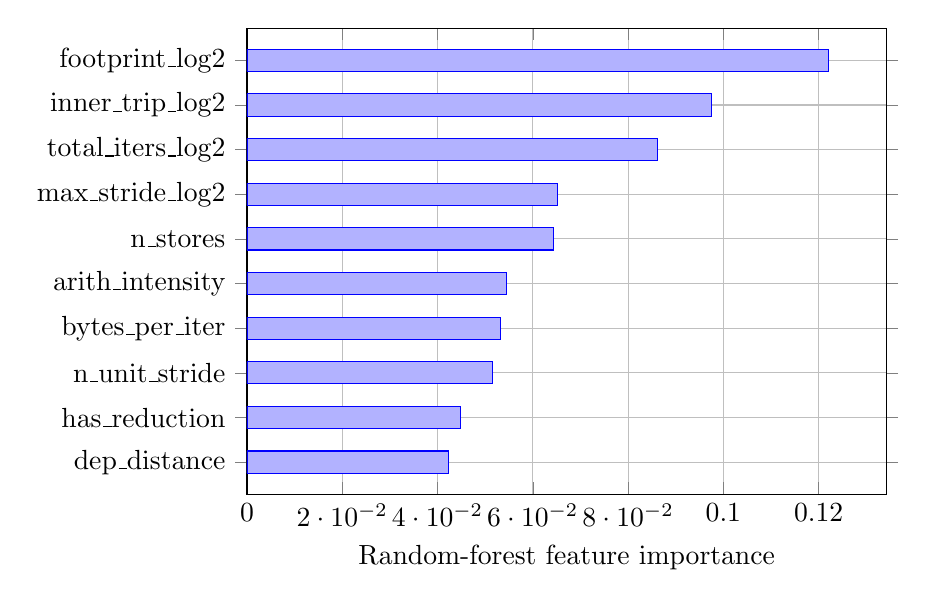
\begin{tikzpicture}
\begin{axis}[
    xbar, width=0.8\textwidth, height=7.5cm,
    xlabel={Random-forest feature importance},
    symbolic y coords={dep\_distance,has\_reduction,n\_unit\_stride,bytes\_per\_iter,arith\_intensity,n\_stores,max\_stride\_log2,total\_iters\_log2,inner\_trip\_log2,footprint\_log2},
    ytick=data, xmin=0, bar width=8pt, enlarge y limits=0.08, grid=major]
\addplot coordinates {(0.0423,dep\_distance) (0.0448,has\_reduction) (0.0515,n\_unit\_stride) (0.0532,bytes\_per\_iter) (0.0545,arith\_intensity) (0.0643,n\_stores) (0.0652,max\_stride\_log2) (0.0861,total\_iters\_log2) (0.0976,inner\_trip\_log2) (0.1220,footprint\_log2)};
\end{axis}
\end{tikzpicture}
\caption{Ten most important loop features.}
\label{fig:importance}
\end{figure}
